\documentclass[11pt]{beamer}
\usetheme{AnnArbor}
\usepackage[utf8]{inputenc}
\usepackage[spanish]{babel}
\usepackage{amsmath}
\usepackage{amsfonts}
\usepackage{amssymb}
\usepackage{graphicx}
\usepackage{lipsum}
\usepackage{ragged2e}

\author{Fabian Sierra Acarapi}
\title[Vida Artificial]{Universidad Nacional "Siglo XX"\\Area: Tecnologia\\Carrera: Ing. Informatica}
\date{4 de diciembre de 2019}
\subtitle{.\\.\\VIDA ARTIFICIAL}
\logo{
\includegraphics[scale=0.2]{unsxx.png}}
%\setbeamercovered{transparent} 
%\setbeamertemplate{navigation symbols}{} 
%\logo{unsxx.png} 
%\institute{} 
%\date{} 
%\subject{aprendiendo} 

\AtBeginSection[]
{
	 \begin{frame}<beamer>{Contenido}
	 	\tableofcontents[currentsection,currentsubsection]
	 \end{frame}
}

\begin{document}

\begin{frame}

\titlepage
		\begin{figure}
		%	\centering
			
			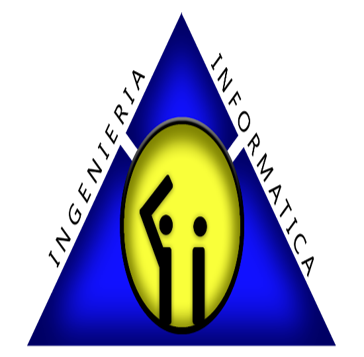
\includegraphics[scale=0.2]{informatica.png}
			
		\end{figure}
%\maketitle

\end{frame}

%\begin{frame}
%\tableofcontents
%\end{frame}

\begin{frame}{Contenido}

	\tableofcontents
\end{frame}



\section{Resumen}
	\begin{frame}{Resumen}
		\justify
		La vida artificial es un desarrollo humano que tiene como objeto de estudio la 			        investigación de la vida y los sistemas artificiales que exhiben propiedades similares                  		a los seres vivos, a través de modelos de simulación. El científico Christopher Langton 		fue el primero en utilizar el término a fines de la década de 1980 cuando se celebró la 		"Primera Conferencia Internacional de la Síntesis y Simulación de Sistemas Vivientes" 			(también conocido como Vida Artificial I) en Laboratorio Nacional de Los Álamos en 				1987. Existen tres tipos principales de vida artificial, nombrados de acuerdo a su 				enfoque: soft, con un enfoque en el software; hard, con un enfoque en el hardware; y 			wet, con un enfoque en la bioquímica.		
			
	
	\end{frame}
\section{Introduccion}
	\begin{frame}{Introduccion}
	\justify
	La Vida Artificial es el estudio de la vida y de los sistemas artificiales que exhiben propiedades 				similares a los seres vivos, a través de modelos de simulación. El científico Christopher Langton fue el 		primero a utilizar el término a fines de los años 1980.
		\begin{figure}
			\centering
			
			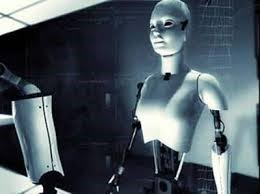
\includegraphics[scale=0.5]{robot.jpg}
			
		\end{figure}
	\end{frame}
\section{Caracteristicas De Campo}
	\begin{frame}{Caracteristicas De Campo}
		\justify
		El campo se caracteriza por el uso extenso de programas informáticos y simulaciones que incluyen cálculo evolutivo (algoritmos evolutivos, algoritmos genéticos (GA por el inglés Genetic Algorithm), programación genética, inteligencia de enjambre, optimización de colonias de hormigas), química artificial, modelos basados en agentes, y autómatas celulares (CA del inglés Cellular Automata). 
aquellas técnicas se ven como sub campos de la vida artificial. 

	\end{frame}
	
	\begin{frame}{Caracteristicas De Campo}
		\justify
		 La vida artificial es un punto de reunión para gente de otros muchos campos más tradicionales como lingüística, física, matemáticas, filosofía, informática, biología, antropología y sociología en los cuales se puede hablar de enfoques computacionales y teóricos inusuales que serian controvertidas dentro de su propia disciplina. 

	\end{frame}
\section{Historia y Contribuciones}
	\begin{frame}{Historia y Contribuciones}
	\justify
	\textbf{ANTES DE LAS COMPUTADORAS}\\
	Uno de los primeros pensadores de la edad moderna que previó los potenciales de la vida artificial, separada de inteligencia artificial, era el prodigio matemático e informático John Von Neumann. En el Simposio Hixon, ofrecido por Linus Carl Pauling en Pasadena, California a finales de los años 40, Von Neumann hizo una conferencia titulada "The General and Logical Theory of Automata" ("La Teoría General y Lógica de Autómatas"). Definía un "autómata" como cualquier máquina cuyo comportamiento provenía de la lógica, paso a paso, combinando información desde el ambiente y su propia programación, y decía que al final se encontrarían organismos naturales que siguieran reglas simples similares. 

	\end{frame}
	
	\begin{frame}{Historia y Contribuciones}
	\justify
	\textbf{ANTES DE LAS COMPUTADORAS}\\
	Von Neumann trabajó en su teoría de autómatas intensivamente hasta el momento de su muerte, y lo consideró su trabajo más importante. Homer Jacobsonilustró la auto replicación de forma básica en los años 50 con un modelo de un grupo de aprendizaje -- un "organismo" semilla que consistía en una "cabeza" y un vagón de "cola" que podían usar sencillas reglas del sistema para crear de forma consistente nuevos "organismos" idénticos a él mismo, siempre y cuanto hubiera un almacén aleatorio de piezas para un nuevo vagón de dónde poder extraer. 


	\end{frame}
	\begin{frame}{Historia y Contribuciones}
	\justify
	\textbf{19870s 1980s}\\
	El erudito en filosofía Arthur Burks, que había trabajado con Von Neumann (y en efecto, organizado sus artículos tras su muerte), encabezaba el Logic of Computers Group (Grupo de Lógica Informática) en la Universidad de Michigan. Devolvió las vistas pasadas por alto del pensador americano del siglo XIX Charles S. Peirce a la edad moderna. 
 

	\end{frame}
\section{Simuladores de organismos digitales/vida artificial}
	\begin{frame}{Simuladores de organismos digitales/vida artificial}
		\justify
		
		\textbf{Basados en programación}\\
Incluyen organismos con un lenguaje DAN complejo , usualmente Turing completo. Estos lenguajes se presentan en la forma de programas de computadora, en lugar de DNA biológico.\\
\textbf{Basados en parámetros}\\
Los organismos son construidos generalmente con comportamientos predefinidos que son afectados por diversos parámetros que mutan. Esto significa que cada organismo contiene una colección de número que cambian y afectan su comportamiento de formas bien definidas. Software de Ventrella Darwin Pond Gene Pool

	\end{frame}
	
	\begin{frame}{Simuladores de organismos digitales/vida artificial}
		\justify
		
		\textbf{Basados en células}\\
Los organismos se construyen como una célula individual, con genes que expresan proteínas. La expresión genética afecta el comportamiento de la célula. El objetivo aquí es usualmente ilustrar las propiedades emergentes de organismos pluricelulares.\\
Cell-O-Sim\\
Kyresoo Plants


Basados en redes neuronales
Estas simulaciones tienen criaturas que aprenden y crecen usando redes neuronales o derivados cercanos. El énfasis suele ponerse más en el crecimiento y el aprendizaje que en la evolución
Creatures
NERO - Neuro Evolving Robotic Operatives
Noble Ape
Polyworld

	\end{frame}
	\begin{frame}{Simuladores de organismos digitales/vida artificial}
		\justify
		
		\textbf{Basados en redes neuronales}\\
Estas simulaciones tienen criaturas que aprenden y crecen usando redes neuronales o derivados cercanos. El énfasis suele ponerse más en el crecimiento y el aprendizaje que en la evolución.\\
Creatures\\
NERO - Neuro Evolving Robotic Operatives\\
Noble Ape\\
Polyworld

	\end{frame}
	
\appendix
\section<presentation>*{Referencias}

\begin{frame}[allowframebreaks]
\frametitle<presentation>{Referencias}

\begin{thebibliography}{10}
	\beamertemplateonlinebibitems
	
	\bibitem{Autor1990}
	Vida artificial
	\newblock{\em En Wikipedia, la enciclopedia libre.}.

	 \newblock{Recuperado de https://es.wikipedia.org vida artificial}

	\beamertemplateonlinebibitems
	
	\bibitem{Autor19901}
	Vida artificial—EcuRed.
	\newblock{\em	Recuperado 29 de noviembre de 2019,}

	\newblock{https: www.ecured.cu Vida artificial}
	
	
\end{thebibliography}
\end{frame}
	
\end{document}